\documentclass[aspectratio=169]{beamer}
\usetheme{Madrid}
\usecolortheme{default}

\usepackage{tikz}
\usetikzlibrary{shapes, arrows, positioning}
\usepackage{amsmath}
\usepackage{amssymb}

\title{Can Math Prove Everything?}
\subtitle{Gödel's Incompleteness Theorems}
\author{Brendan Shea, PhD}
\institute{Rochester Community and Technical College}
\date{}

\begin{document}

% Slide 1: Title Slide
\begin{frame}
\titlepage
\begin{center}
\textit{Gödel's Mind-Bending Discovery}
\end{center}
\end{frame}

% Slide 2: The Big Question
\begin{frame}{The Big Question}

\begin{alertblock}{A Mathematical Revolution}
In 1931, a 25-year-old mathematician named Kurt Gödel published a paper that would forever change our understanding of mathematics.
\end{alertblock}

\begin{itemize}
    \item Can we create a perfect system of mathematics that can prove all true statements?
    \item For centuries, mathematicians believed this goal was achievable.
    \item Gödel discovered something shocking: the answer is no.
    \item Today, we'll explore why this "impossible" result is actually true.
\end{itemize}

\end{frame}

% Slide 3: What We'll Discover Today
\begin{frame}{What We'll Discover Today}

\begin{itemize}
    \item We'll journey through the foundations of logic, mathematical systems, and the power of self-reference.
    \item We'll meet brilliant thinkers like David Hilbert and Kurt Gödel who changed how we understand mathematics.
    \item We'll understand why some truths can never be proven within a logical system.
    \item We'll see how Gödel's discovery impacts mathematics, computer science, and philosophy.
\end{itemize}

\vspace{0.5cm}
\begin{center}
\textbf{Warning:} This material is challenging, but the journey is worth it!
\end{center}

\end{frame}

% Slide 4: What is Logic?
\begin{frame}{What is Logic?}

\begin{itemize}
    \item \textbf{Logic} is the study of valid reasoning and correct argumentation.
    \item Logic helps us distinguish good arguments from bad ones using precise rules.
    \item Mathematical logic applies these principles to mathematical statements and proofs.
\end{itemize}

\begin{block}{A Simple Logical Argument}
\begin{enumerate}
    \item Premise 1: All cats are animals.
    \item Premise 2: Fluffy is a cat.
    \item Conclusion: Therefore, Fluffy is an animal.
\end{enumerate}
This argument is \textit{logically valid}—if the premises are true, the conclusion must be true.
\end{block}

\end{frame}

% Slide 5: Statements That Are True or False
\begin{frame}{Statements That Are True or False}

\begin{itemize}
    \item In mathematics, we work with statements that are objectively either true or false.
    \item A \textbf{mathematical statement} is a declarative sentence that has a definite truth value.
    \item Not all sentences qualify as mathematical statements—opinions and questions don't count.
\end{itemize}

\begin{table}
\centering
\begin{tabular}{|l|c|l|}
\hline
\textbf{Statement} & \textbf{Truth Value} & \textbf{Type} \\
\hline
$2 + 2 = 4$ & TRUE & Mathematical \\
$2 + 2 = 5$ & FALSE & Mathematical \\
This pizza is delicious & ??? & Opinion (not math) \\
Is $x > 0$? & ??? & Question (not a statement) \\
\hline
\end{tabular}
\end{table}

\end{frame}

% Slide 6: What is a Proof?
\begin{frame}{What is a Proof?}

\begin{itemize}
    \item A \textbf{proof} is a step-by-step logical argument that establishes the truth of a mathematical statement.
    \item Proofs start from things we already accept as true, called axioms or previously proven theorems.
    \item Each step in a proof follows from logical rules that preserve truth.
    \item A valid proof gives us 100\% certainty—not just strong evidence, but absolute logical necessity.
\end{itemize}

\begin{block}{The Power of Proof}
Unlike scientific theories that can be revised with new evidence, a mathematical proof is forever true. Once proven, always proven!
\end{block}

\end{frame}

% Slide 7: Simple Proof Example
\begin{frame}{Simple Proof Example}

\begin{itemize}
    \item Let's see a proof in action to understand how rigorous reasoning works.
    \item We'll prove: \textit{If $x + 3 = 7$, then $x = 4$}.
\end{itemize}

\begin{block}{Proof}
\begin{align*}
\text{Given:} \quad & x + 3 = 7 \\
\text{Step 1:} \quad & \text{Subtract 3 from both sides} \\
& x + 3 - 3 = 7 - 3 \\
\text{Step 2:} \quad & \text{Simplify both sides} \\
& x = 4 \\
\text{Conclusion:} \quad & \text{Therefore, } x = 4 \quad \blacksquare
\end{align*}
\end{block}

\begin{itemize}
    \item This is bulletproof reasoning—each step is justified and leads inevitably to the conclusion.
\end{itemize}

\end{frame}

% Slide 8: Axioms: The Starting Rules
\begin{frame}{Axioms: The Starting Rules}

\begin{itemize}
    \item \textbf{Axioms} are basic truths that we accept without proof—they are our starting points.
    \item Every mathematical system must begin somewhere, with statements we agree to take as self-evidently true.
    \item Axioms are like the rules of a game: we establish them first, then see what follows from them.
    \item The question Gödel explored: Can we choose a perfect set of axioms that proves everything?
\end{itemize}

\begin{block}{Example Axiom: Transitivity of Equality}
If $a = b$ and $b = c$, then $a = c$.
\end{block}

\end{frame}

% Slide 9: The Dream of Perfect Mathematics
\begin{frame}{The Dream of Perfect Mathematics}

\begin{itemize}
    \item By the early 1900s, mathematicians had developed a bold and ambitious vision for the future.
    \item They dreamed of creating one complete set of axioms from which every true mathematical statement could be proven.
    \item If successful, mathematics would become a "finished" system—perfect, complete, and unassailable.
    \item This wasn't just about solving problems; it was about achieving absolute certainty in human knowledge.
\end{itemize}

\begin{alertblock}{The Ultimate Goal}
Mathematics would be transformed into a purely mechanical process: feed in axioms, turn the logical crank, and out comes every mathematical truth!
\end{alertblock}

\end{frame}

% Slide 10: Meet David Hilbert
\begin{frame}{Meet David Hilbert (1862--1943)}

\begin{itemize}
    \item David Hilbert was one of the most influential mathematicians of all time.
    \item He made groundbreaking contributions to geometry, algebra, mathematical physics, and logic.
    \item In the 1920s, Hilbert launched an ambitious research program to secure the foundations of mathematics.
    \item He famously declared: "We must know, we will know!"—expressing absolute confidence in mathematics.
\end{itemize}

\begin{block}{Hilbert's Vision}
Hilbert believed that with the right axioms and logical rules, we could create a mathematical system that was both complete (proves all truths) and consistent (proves no contradictions).
\end{block}

\end{frame}

% Slide 11: The Hilbert Program Goals
\begin{frame}{The Hilbert Program: Three Goals}

\textbf{Hilbert's Program} aimed to establish three essential properties for mathematics:

\begin{enumerate}
    \item \textbf{Completeness}: Every true mathematical statement can be proven from the axioms.
    \begin{itemize}
        \item If something is true, we should be able to prove it.
    \end{itemize}
    \item \textbf{Consistency}: The system never proves contradictions—no statement is both true and false.
    \begin{itemize}
        \item Mathematics must never contradict itself.
    \end{itemize}
    \item \textbf{Decidability}: There exists a mechanical procedure to determine whether any statement is provable.
    \begin{itemize}
        \item We should have an algorithm that always tells us yes or no.
    \end{itemize}
\end{enumerate}

\vspace{0.3cm}
\textit{This seemed achievable... until Kurt Gödel entered the scene.}

\end{frame}

% Slide 12: Enter Kurt Gödel
\begin{frame}{Enter Kurt Gödel (1906--1978)}

\begin{itemize}
    \item Kurt Gödel was born in 1906 in Brünn, Austria-Hungary (now Brno, Czech Republic).
    \item He was a brilliant student with an intense curiosity about mathematics and philosophy.
    \item Gödel studied at the University of Vienna, where he joined the famous "Vienna Circle" of philosophers.
    \item In 1931, at just 25 years old, he published a paper that would shatter Hilbert's dream.
\end{itemize}

\begin{block}{The Breakthrough}
Gödel's incompleteness theorems proved that Hilbert's goals were fundamentally impossible to achieve—not because we weren't smart enough, but because of deep logical limitations built into mathematics itself.
\end{block}

\end{frame}

% Slide 13: Discussion Questions - Set 1
\begin{frame}{Discussion Break: Questions to Consider}

\begin{block}{Take a moment to think about these questions:}
\begin{enumerate}
    \item Why would mathematicians want a "complete" system? What would be the benefits of being able to prove everything?
    \item Can you think of other systems with rules (like games, legal systems, or grammar)? Are any of them complete?
    \item If we could prove every truth in mathematics, what would that mean for mathematics as a field of study? Would there be anything left to discover?
\end{enumerate}
\end{block}

\vspace{0.5cm}
\begin{center}
\textit{Jot down your thoughts—we'll discuss some answers together!}
\end{center}

\end{frame}

% Slide 14: What is a Formal System?
\begin{frame}{What is a Formal System?}

\begin{itemize}
    \item A \textbf{formal system} is a precisely defined mathematical framework consisting of symbols, axioms, and rules.
    \item Think of it as a sophisticated game with completely precise rules—no ambiguity allowed.
    \item Formal systems allow us to study mathematics in a rigorous, mechanical way.
\end{itemize}

\begin{block}{Components of a Formal System}
\begin{enumerate}
    \item \textbf{Symbols}: The alphabet we use (like numbers, $+$, $=$, variables)
    \item \textbf{Axioms}: The starting truths we accept without proof
    \item \textbf{Rules of Inference}: Logical rules for deriving new statements from old ones
\end{enumerate}
\end{block}

\end{frame}

% Slide 15: Example: A Tiny Formal System
\begin{frame}{Example: A Tiny Formal System}

\begin{itemize}
    \item Let's create a simple formal system to see how they work in practice.
    \item This will help us understand how mathematicians build up knowledge from basic principles.
\end{itemize}

\begin{block}{Our Miniature System}
\textbf{Symbols:} $0, 1, 2, 3, \ldots, +, =$

\textbf{Axioms:} $1 + 1 = 2$ and $2 + 1 = 3$

\textbf{Rule:} If $a = b$, then $a + c = b + c$ (can add the same thing to both sides)
\end{block}

\begin{itemize}
    \item From axiom $1 + 1 = 2$, we can add $1$ to both sides: $1 + 1 + 1 = 2 + 1$
    \item Using our second axiom, we get: $1 + 1 + 1 = 3$ (a new fact we derived!)
\end{itemize}

\end{frame}

% Slide 16: Consistent vs. Inconsistent
\begin{frame}{Consistent vs. Inconsistent Systems}

\begin{itemize}
    \item A \textbf{consistent system} never proves contradictions—it cannot prove that a statement is both true and false.
    \item An \textbf{inconsistent system} can prove contradictions, which is catastrophic for mathematics.
    \item In an inconsistent system, you can actually prove anything at all, even complete nonsense!
\end{itemize}

\begin{alertblock}{Example of Inconsistency}
Imagine a system that proves: "All numbers are even" AND "Some numbers are odd" AND "There is only one number."

This system is broken—once you have a contradiction, logic falls apart and every statement becomes "provable."
\end{alertblock}

\end{frame}

% Slide 17: Complete vs. Incomplete
\begin{frame}{Complete vs. Incomplete Systems}

\begin{itemize}
    \item A \textbf{complete system} is one in which every true statement can be proven using the axioms and rules.
    \item An \textbf{incomplete system} contains true statements that cannot be proven within the system itself.
    \item Before Gödel, mathematicians hoped that mathematical systems could be both complete and consistent.
\end{itemize}

\begin{block}{Thought Experiment}
Try to imagine a mathematical fact that is definitely true, but that you could never prove is true using your system's rules. Does such a thing seem possible? Could it even exist?
\end{block}

\begin{itemize}
    \item This is exactly what Gödel discovered—such statements not only exist, they must exist in any sufficiently powerful system!
\end{itemize}

\end{frame}

% Slide 18: Self-Reference: The Trickster
\begin{frame}{Self-Reference: The Trickster}

\begin{itemize}
    \item \textbf{Self-reference} occurs when something refers to or describes itself.
    \item Self-reference appears harmless but can create logical paradoxes and puzzles.
    \item Gödel's genius was recognizing that self-reference could be built into mathematical statements.
\end{itemize}

\begin{block}{Examples of Self-Reference}
\begin{itemize}
    \item "This sentence has five words." (It refers to itself and is true!)
    \item "This sentence is false." (The Liar's Paradox—if true, then false; if false, then true!)
    \item "Do not read this sentence." (You just did!)
\end{itemize}
\end{block}

\end{frame}

% Slide 19: The Barber Paradox
\begin{frame}{The Barber Paradox}

\begin{block}{The Setup}
In a village, there is a barber who shaves all and only those men who do not shave themselves.

\textbf{Question:} Does the barber shave himself?
\end{block}

\begin{itemize}
    \item \textbf{If yes} (the barber shaves himself): Then he's someone who shaves himself, so according to the rule, he shouldn't shave himself. Contradiction!
    \item \textbf{If no} (the barber doesn't shave himself): Then he's someone who doesn't shave himself, so according to the rule, the barber should shave him. Contradiction!
    \item Self-reference has created an impossible, paradoxical situation where neither answer works.
    \item This is the kind of logical trap Gödel would exploit in mathematics itself!
\end{itemize}

\end{frame}

% Slide 20: Why Self-Reference Matters
\begin{frame}{Why Self-Reference Matters for Gödel}

\begin{center}
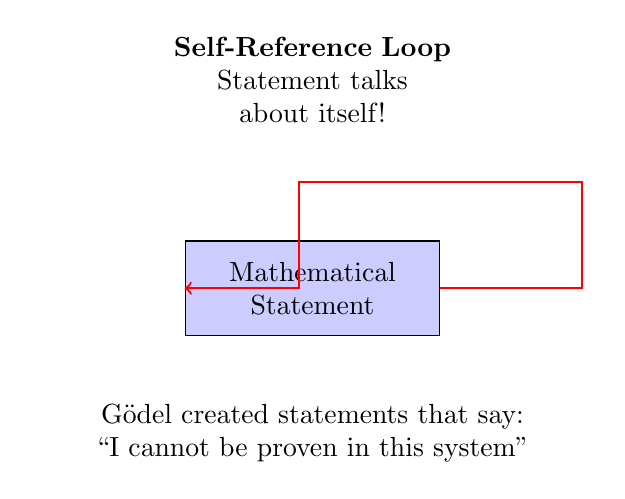
\begin{tikzpicture}[scale=0.9]
    % Central idea
    \node[rectangle, draw, fill=blue!20, text width=3cm, align=center, minimum height=1.2cm] (statement) at (0,0) {Mathematical Statement};
    
    % Arrow looping back
    \draw[->, thick, red] (statement.east) -- ++(2,0) -- ++(0,1.5) -- ++(-4,0) -- ++(0,-1.5) -- (statement.west);
    
    \node[above, text width=4cm, align=center] at (0,2.2) {\textbf{Self-Reference Loop}\\Statement talks about itself!};
    
    % Bottom labels
    \node[below, text width=7cm, align=center] at (0,-1.5) {Gödel created statements that say:\\``I cannot be proven in this system''};
\end{tikzpicture}
\end{center}

\begin{itemize}
    \item Self-reference breaks normal logical reasoning and creates paradoxes.
    \item Gödel's brilliant insight: Apply self-reference to mathematics itself, not just to everyday language.
    \item The key to his proof would be constructing a mathematical statement that refers to its own provability.
\end{itemize}

\end{frame}

% Slide 21: Gödel's Brilliant Idea
\begin{frame}{Gödel's Brilliant Idea}

\begin{itemize}
    \item Gödel asked a revolutionary question: What if a mathematical statement could talk about itself?
    \item Imagine a statement that says: "This statement cannot be proven."
    \item Now think carefully: Is that statement true? Can it be proven?
    \item This self-referential twist is the key to everything Gödel discovered!
\end{itemize}

\begin{alertblock}{The Crucial Insight}
If we can make a mathematical statement say "I cannot be proven," we can create a paradox similar to the Barber Paradox—but this time, inside mathematics itself!
\end{alertblock}

\end{frame}

% Slide 22: Gödel Numbering: Turning Math into Numbers
\begin{frame}{Gödel Numbering: Turning Math into Numbers}

\begin{itemize}
    \item Gödel's first challenge: How can a mathematical statement refer to itself?
    \item His ingenious solution: Assign a unique number to every mathematical symbol and statement.
    \item This process is called \textbf{Gödel numbering}, and it allows statements to be coded as numbers.
\end{itemize}

\begin{block}{Example Coding Scheme}
\begin{tabular}{cccccc}
Symbol: & ``0'' & ``1'' & ``+'' & ``='' & ``('' \\
Number: & 1 & 2 & 3 & 4 & 5
\end{tabular}

\vspace{0.3cm}
Using this scheme, the statement ``$0 + 1$'' could be encoded as the number $132$.

Different symbols combine to create unique numbers for every possible mathematical statement!
\end{block}

\end{frame}

% Slide 23: Why Number Mathematical Statements?
\begin{frame}{Why Number Mathematical Statements?}

\begin{itemize}
    \item Once statements are numbers, mathematical statements can refer to other statements by using their numbers.
    \item Even more mind-bending: A statement can refer to itself using its own Gödel number!
    \item This is like giving every sentence in a book a unique ID number, then writing sentence \#847 to say "The sentence with ID \#847 is false"—and that sentence is \#847!
\end{itemize}

\begin{block}{The Power of Numbering}
By turning statements into numbers, Gödel made mathematics capable of talking about itself. Mathematical statements could now discuss whether other statements (or even themselves!) can be proven.
\end{block}

\end{frame}

% Slide 24: Creating the Self-Referential Statement
\begin{frame}{Creating the Self-Referential Statement}

\begin{center}
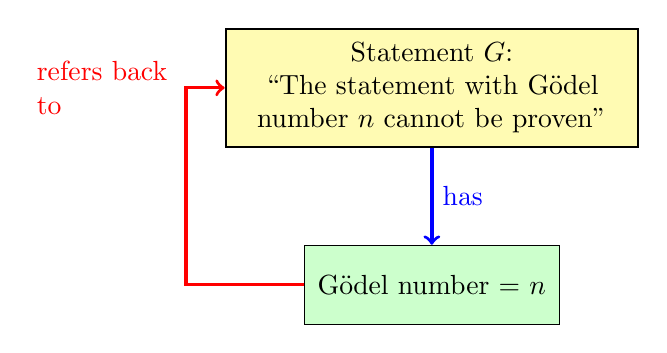
\begin{tikzpicture}[scale=1.0]
    % The G statement box
    \node[rectangle, draw, fill=yellow!30, text width=5cm, align=center, minimum height=1.5cm, thick] (G) at (0,0) {Statement $G$:\\``The statement with Gödel\\number $n$ cannot be proven''};
    
    % The number box
    \node[rectangle, draw, fill=green!20, text width=3cm, align=center, minimum height=1cm] (num) at (0,-2.5) {Gödel number = $n$};
    
    % Arrows showing the self-reference
    \draw[->, very thick, blue] (G.south) -- (num.north) node[midway, right] {has};
    \draw[->, very thick, red] (num.west) -- ++(-1.5,0) -- ++(0,2.5) -- (G.west) node[midway, left, text width=2cm] {refers back to};
\end{tikzpicture}
\end{center}

\begin{itemize}
    \item Gödel constructed statement $G$ to say: "I cannot be proven in this system."
    \item This is mathematical inception—a statement that loops back to describe itself!
\end{itemize}

\end{frame}


% Slide 25: The Setup is Complete
\begin{frame}{The Setup is Complete}

\begin{itemize}
    \item We now have all the pieces Gödel needed for his revolutionary proof.
    \item Let's review what we've assembled before we see the mind-bending conclusion.
\end{itemize}

\begin{block}{Gödel's Toolkit}
\begin{enumerate}
    \item A formal system for mathematics with axioms and rules
    \item Gödel numbering: a way to turn statements into numbers
    \item Statement $G$: a self-referential statement that says "I cannot be proven"
    \item The question: What happens when we try to prove or disprove $G$?
\end{enumerate}
\end{block}

\begin{itemize}
    \item Everything is in place—now comes the brilliant logical argument that changed mathematics forever.
\end{itemize}

\end{frame}

% Slide 26: Discussion Questions - Set 2
\begin{frame}{Discussion Break: Questions to Consider}

\begin{block}{Take a moment to think about these questions:}
\begin{enumerate}
    \item Try to explain Gödel numbering to someone in your own words. Why is it such a clever technique?
    \item Before we reveal the answer: What do you think happens with statement $G$? Can it be proven? Is it true?
    \item Have you encountered self-reference in other contexts—in art, literature, movies, or everyday life? Share an example.
\end{enumerate}
\end{block}

\vspace{0.5cm}
\begin{center}
\textit{Think carefully about statement $G$—the next section reveals the answer!}
\end{center}

\end{frame}

% Slide 27: Analyzing Statement G
\begin{frame}{Analyzing Statement G}

\begin{itemize}
    \item Remember: Statement $G$ says "I cannot be proven in this system."
    \item There are only two logical possibilities we need to consider.
    \item Let's carefully examine each possibility and see where the logic leads us.
\end{itemize}

\begin{block}{Two Possibilities}
\begin{enumerate}
    \item \textbf{Possibility 1:} Statement $G$ is provable in our system.
    \item \textbf{Possibility 2:} Statement $G$ is not provable in our system.
\end{enumerate}
One of these must be true—there's no third option!
\end{block}

\begin{itemize}
    \item We'll explore each scenario and discover something remarkable about the nature of mathematical truth.
\end{itemize}

\end{frame}

% Slide 28: Scenario 1 - If G IS Provable
\begin{frame}{Scenario 1: If $G$ IS Provable}

\begin{alertblock}{Following the Logic}
Suppose we can prove $G$ in our system. What would this mean?
\end{alertblock}

\begin{itemize}
    \item If we can prove $G$, then what $G$ says must be true (proofs only establish true things in consistent systems).
    \item But $G$ says "I cannot be proven"—that's what $G$ claims!
    \item Wait—we just assumed we CAN prove $G$, but $G$ says we CAN'T prove it!
    \item This is a contradiction! Our system has just proven something false.
    \item If this happens, our system is \textbf{inconsistent}—it proves falsehoods, and we can't trust it.
\end{itemize}

\end{frame}

% Slide 29: Scenario 2 - If G is NOT Provable
\begin{frame}{Scenario 2: If $G$ is NOT Provable}

\begin{alertblock}{The Other Path}
Now suppose we cannot prove $G$ in our system. What does this tell us?
\end{alertblock}

\begin{itemize}
    \item If we cannot prove $G$, then what $G$ says is actually true!
    \item Remember, $G$ says "I cannot be proven"—and that's exactly the situation we're in.
    \item So $G$ is a TRUE statement about our mathematical system.
    \item But we just said we can't prove it—so $G$ is true but unprovable!
    \item We've discovered a true mathematical statement that cannot be proven within our system.
\end{itemize}

\end{frame}

% Slide 30: The Inescapable Conclusion
\begin{frame}{The Inescapable Conclusion}

\begin{center}
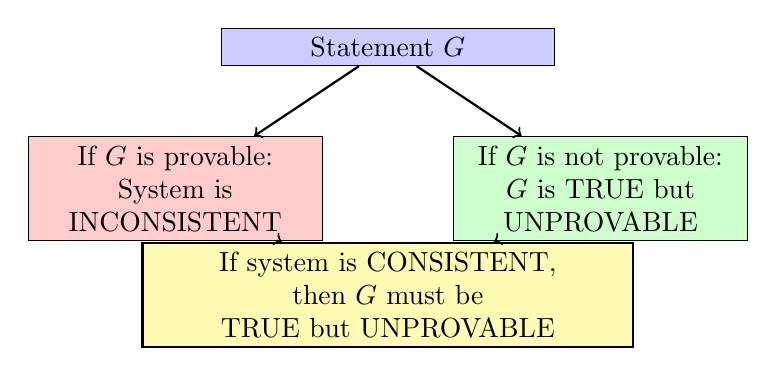
\begin{tikzpicture}[scale=0.9]
    % Top node
    \node[rectangle, draw, fill=blue!20, text width=4cm, align=center] (start) at (0,3) {Statement $G$};
    
    % Left branch
    \node[rectangle, draw, fill=red!20, text width=3.5cm, align=center] (left) at (-3,1) {If $G$ is provable:\\System is\\INCONSISTENT};
    
    % Right branch
    \node[rectangle, draw, fill=green!20, text width=3.5cm, align=center] (right) at (3,1) {If $G$ is not provable:\\$G$ is TRUE but\\UNPROVABLE};
    
    % Bottom conclusion
    \node[rectangle, draw, fill=yellow!30, text width=6cm, align=center, thick] (bottom) at (0,-0.5) {If system is CONSISTENT,\\then $G$ must be\\TRUE but UNPROVABLE};
    
    \draw[->, thick] (start) -- (left);
    \draw[->, thick] (start) -- (right);
    \draw[->, thick] (left) -- (bottom);
    \draw[->, thick] (right) -- (bottom);
\end{tikzpicture}
\end{center}

\begin{itemize}
    \item If we want a consistent system (one that doesn't prove falsehoods), then we must accept that $G$ is true but unprovable!
\end{itemize}

\end{frame}

% Slide 31: The First Incompleteness Theorem
\begin{frame}{The First Incompleteness Theorem}

\begin{alertblock}{Gödel's First Incompleteness Theorem (1931)}
In any consistent formal system that is powerful enough to describe basic arithmetic, there exist statements that are true but cannot be proven within that system.
\end{alertblock}

\begin{itemize}
    \item Translation: Mathematics will always have true statements that it cannot prove!
    \item The system is necessarily \textbf{incomplete}—there are truths beyond its reach.
    \item This isn't because we chose the wrong axioms or aren't smart enough.
    \item It's impossible in principle—a fundamental limitation built into the structure of logic itself.
\end{itemize}

\end{frame}

% Slide 32: What This Means
\begin{frame}{What This Means}

\begin{itemize}
    \item Mathematics cannot prove all truths about itself, no matter how we set it up.
    \item There will always be "blind spots"—true statements that slip through the cracks.
    \item This applies to any formal system powerful enough to do basic arithmetic.
    \item Even if we add new axioms to prove $G$, new unprovable statements will appear!
\end{itemize}

\begin{block}{An Important Clarification}
This doesn't mean we can never know these statements are true. We can reason about them from outside the system (as Gödel did!). But the system itself cannot prove them using only its own rules.
\end{block}

\end{frame}

% Slide 33: The Second Incompleteness Theorem
\begin{frame}{The Second Incompleteness Theorem}

\begin{itemize}
    \item Gödel didn't stop with just one earth-shattering theorem—he proved something even more shocking.
    \item His second theorem deals with a system's ability to verify its own reliability.
\end{itemize}

\begin{alertblock}{Gödel's Second Incompleteness Theorem}
No consistent formal system can prove its own consistency.
\end{alertblock}

\begin{itemize}
    \item In other words: Mathematics cannot prove that mathematics doesn't contradict itself!
    \item It's like asking someone "Can you prove you're not crazy?"—they can't really give a convincing proof using only their own reasoning.
    \item A system cannot bootstrap itself to verify its own trustworthiness.
\end{itemize}

\end{frame}

% Slide 34: Why Can't We Prove Consistency?
\begin{frame}{Why Can't We Prove Consistency?}

\begin{itemize}
    \item Here's the logical trap: suppose a system could prove its own consistency.
    \item If the system proves it's consistent, then it proves "$G$ cannot be proven" (because consistency implies $G$ is unprovable).
    \item But proving "$G$ cannot be proven" is essentially the same as proving $G$ itself!
    \item We already showed that proving $G$ leads to inconsistency—a contradiction.
\end{itemize}

\begin{block}{The Paradox}
\begin{center}
If a system proves its consistency $\Rightarrow$ It proves $G$ $\Rightarrow$ Contradiction!

Therefore: No consistent system can prove its own consistency.
\end{center}
\end{block}

\end{frame}

% Slide 35: The Collapse of Hilbert's Dream
\begin{frame}{The Collapse of Hilbert's Dream}

\begin{itemize}
    \item Recall that Hilbert wanted mathematics to be complete, consistent, and decidable.
    \item Gödel's theorems showed that these goals are fundamentally incompatible.
    \item Mathematics has inherent limitations built into its logical structure.
\end{itemize}

\begin{table}
\centering
\begin{tabular}{|l|c|l|}
\hline
\textbf{Hilbert's Goal} & \textbf{Status} & \textbf{Gödel's Result} \\
\hline
Completeness & X & First Incompleteness Theorem \\
Prove Consistency & X & Second Incompleteness Theorem \\
Decidability & X & Related work (Turing, Church) \\
\hline
\end{tabular}
\end{table}

\begin{itemize}
    \item The dream of a perfect, complete mathematical system was impossible from the start.
\end{itemize}

\end{frame}

% Slide 36: What Gödel Did NOT Prove
\begin{frame}{What Gödel Did NOT Prove}

\begin{alertblock}{Important: Avoiding Misunderstandings}
Gödel's theorems are often misinterpreted. Let's be clear about what they do NOT say.
\end{alertblock}

\begin{itemize}
    \item Gödel did NOT prove that mathematics is broken, useless, or unreliable.
    \item Most of mathematics works perfectly fine—we prove countless theorems every day.
    \item The unprovable statements are exotic, unusual cases that rarely affect normal mathematical work.
    \item Gödel did NOT prove that "nothing can be known" or that "truth is relative."
    \item Mathematics is still powerful and trustworthy—it's just not omnipotent or perfectly self-contained.
\end{itemize}

\end{frame}

% Slide 37: An Analogy: The Map Problem
\begin{frame}{An Analogy: The Perfect Map}

\begin{center}
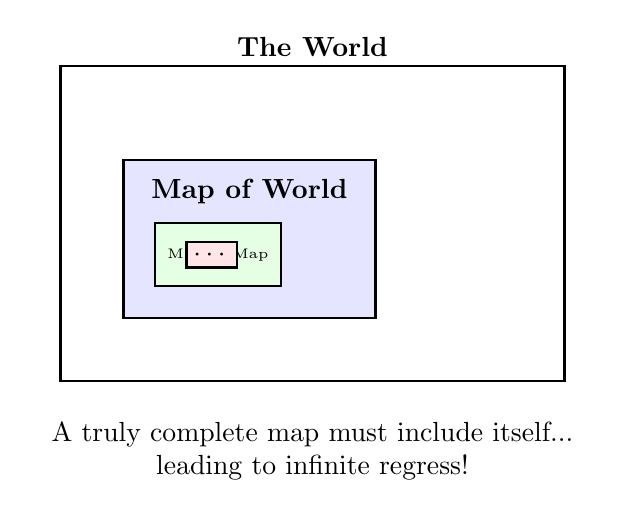
\begin{tikzpicture}[scale=0.8]
    % Outer rectangle (the world)
    \draw[thick] (0,0) rectangle (8,5);
    \node[above] at (4,5) {\textbf{The World}};
    
    % Inner rectangle (the map)
    \draw[thick, fill=blue!10] (1,1) rectangle (5,3.5);
    \node at (3,3) {\textbf{Map of World}};
    
    % Even smaller rectangle (map within map)
    \draw[thick, fill=green!10] (1.5,1.5) rectangle (3.5,2.5);
    \node[font=\tiny] at (2.5,2) {Map of Map};
    
    % Tiny rectangle
    \draw[thick, fill=red!10] (2,1.8) rectangle (2.8,2.2);
    
    % Dots suggesting infinite regress
    \node at (2.4,2) {$\cdots$};
    
    \node[below, text width=7cm, align=center] at (4,-0.5) {A truly complete map must include itself...\\leading to infinite regress!};
\end{tikzpicture}
\end{center}

\begin{itemize}
    \item Perfect self-reference leads to impossible infinite regress.
    \item Mathematics faces a similar limitation when trying to fully describe itself.
\end{itemize}

\end{frame}

% Slide 38: Discussion Questions - Set 3
\begin{frame}{Discussion Break: Questions to Consider}

\begin{block}{Take a moment to think about these questions:}
\begin{enumerate}
    \item How does Gödel's theorem make you feel about mathematics? Does it make math seem less certain, or perhaps more fascinating and mysterious?
    \item Can you think of other systems (legal, scientific, philosophical) that might have similar limitations in "seeing" themselves completely?
    \item Does the inability to prove everything make mathematics less reliable or trustworthy? Why or why not?
\end{enumerate}
\end{block}

\vspace{0.5cm}
\begin{center}
\textit{Reflect on how completeness and truth relate to each other!}
\end{center}

\end{frame}

% Slide 39: Impact on Mathematics
\begin{frame}{Impact on Mathematics}

\begin{itemize}
    \item Mathematicians had to fundamentally rethink the nature of their field after Gödel.
    \item The realization: There can never be a "final theory" that explains everything in mathematics.
    \item Mathematics is an endless frontier—there will always be new questions and mysteries to explore.
    \item This is actually exciting! Mathematics can never be "finished" or exhausted.
\end{itemize}

\begin{block}{A New Perspective}
Rather than seeing incompleteness as a failure, mathematicians came to view it as a feature of mathematics that ensures perpetual discovery and exploration. There will always be more to learn!
\end{block}

\end{frame}

% Slide 40: Impact on Computer Science
\begin{frame}{Impact on Computer Science}

\begin{itemize}
    \item Alan Turing, inspired by Gödel's work, discovered similar limitations in computation.
    \item The \textbf{Halting Problem}: No program can determine whether all other programs will finish running or loop forever.
    \item This is directly analogous to Gödel's incompleteness—some computational questions are undecidable.
    \item There are fundamental limits to what computers can do, no matter how powerful they become.
\end{itemize}

\begin{block}{Parallel Limitations}
\begin{center}
\begin{tabular}{l|l}
\textbf{Mathematics} & \textbf{Computer Science} \\
\hline
Some statements unprovable & Some problems undecidable \\
Can't prove consistency & Can't solve halting problem \\
\end{tabular}
\end{center}
\end{block}

\end{frame}

% Slide 41: Impact on Artificial Intelligence
\begin{frame}{Impact on Artificial Intelligence}

\begin{itemize}
    \item Gödel's work raises profound questions about the nature of mind and machine.
    \item Some philosophers argue: Gödel's theorem shows human minds transcend purely mechanical systems.
    \item Other philosophers counter: Humans are subject to the same logical limitations as machines.
    \item The debate continues today in AI research and philosophy of mind!
\end{itemize}

\begin{block}{The Central Question}
Can machines truly "think" like humans? Or do Gödel's insights about formal systems reveal a fundamental difference between human reasoning and computational processes?
\end{block}

\end{frame}

% Slide 42: Philosophical Question: Truth vs. Proof
\begin{frame}{Truth vs. Proof: A Fundamental Distinction}

\begin{itemize}
    \item Before Gödel, many assumed that mathematical truth and provability were the same thing.
    \item Gödel revealed these are fundamentally different concepts that don't always align.
\end{itemize}

\begin{center}
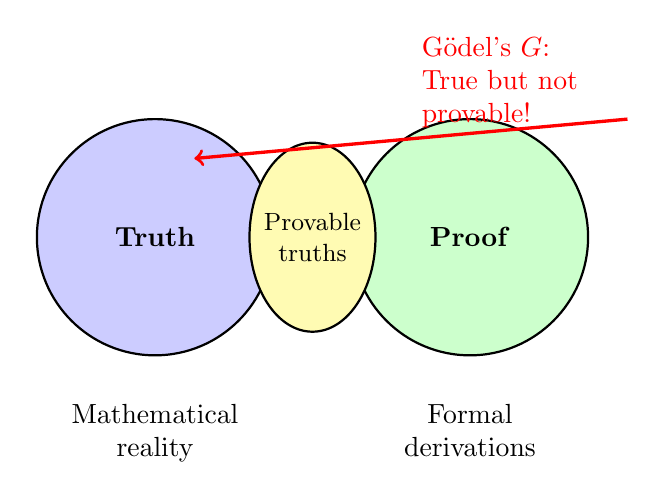
\begin{tikzpicture}[scale=1.0]
    % Truth circle
    \draw[thick, fill=blue!20] (-2,0) circle (1.5cm);
    \node at (-2,0) {\textbf{Truth}};
    \node[below, text width=3cm, align=center] at (-2,-2) {Mathematical\\reality};
    
    % Proof circle
    \draw[thick, fill=green!20] (2,0) circle (1.5cm);
    \node at (2,0) {\textbf{Proof}};
    \node[below, text width=3cm, align=center] at (2,-2) {Formal\\derivations};
    
    % Overlap region
    \draw[thick, fill=yellow!30] (0,0) ellipse (0.8cm and 1.2cm);
    \node[text width=2cm, align=center, font=\small] at (0,0) {Provable\\truths};
    
    % Arrow pointing to the truth circle outside overlap
    \draw[->, very thick, red] (4,1.5) -- (-1.5,1) node[midway, above right, text width=2.5cm] {Gödel's $G$:\\True but not provable!};
\end{tikzpicture}
\end{center}

\end{frame}

% Slide 43: The Limits of Logic
\begin{frame}{The Limits of Logic}

\begin{itemize}
    \item Logic and formal reasoning are incredibly powerful tools for understanding the world.
    \item However, Gödel showed that logic has inherent boundaries that cannot be crossed.
    \item We cannot escape these limitations by being smarter or working harder.
    \item These boundaries are built into the very nature of self-referential systems.
\end{itemize}

\begin{block}{A Lesson in Humility}
Some questions may have no answer within a given system. Some truths may be forever beyond formal proof. This doesn't mean we give up—it means we recognize the scope and limits of our methods and remain intellectually humble.
\end{block}

\end{frame}

% Slide 44: Gödel's Later Life
\begin{frame}{Gödel's Later Life (1906--1978)}

\begin{itemize}
    \item In 1940, Gödel emigrated to the United States to escape World War II and settled in Princeton.
    \item He worked at the Institute for Advanced Study alongside Albert Einstein, becoming close friends.
    \item Einstein once said he went to his office "just to have the privilege of walking home with Gödel."
    \item Sadly, Gödel struggled with paranoia and health issues in his later years, passing away in 1978.
\end{itemize}

\begin{block}{A Lasting Friendship}
The friendship between Einstein (who revolutionized physics) and Gödel (who revolutionized logic) represents one of the most remarkable intellectual partnerships in history.
\end{block}

\end{frame}

% Slide 45: Gödel's Legacy
\begin{frame}{Gödel's Legacy}

\begin{itemize}
    \item Gödel's incompleteness theorems rank among the most important logical discoveries in human history.
    \item His work fundamentally changed mathematics, philosophy, computer science, and cognitive science.
    \item He demonstrated the power of creative, "diagonal" thinking—approaching problems from unexpected angles.
    \item Gödel reminded us that the universe contains deep mysteries that may forever elude complete understanding.
\end{itemize}

\begin{alertblock}{Enduring Influence}
Over 90 years after publication, Gödel's theorems continue to inspire new research and philosophical debates. His insights remain as relevant today as they were in 1931.
\end{alertblock}

\end{frame}

% Slide 46: Why This Matters to You
\begin{frame}{Why This Matters to You}

\begin{itemize}
    \item \textbf{Critical Thinking}: Question assumptions about completeness and absolute certainty in any system.
    \item \textbf{Creativity}: Sometimes the answer to a problem requires thinking outside the system entirely.
    \item \textbf{Humility}: Even our most rigorous and powerful systems have fundamental limitations.
    \item \textbf{Wonder}: Reality is deeper, stranger, and more mysterious than it initially appears.
\end{itemize}

\begin{block}{Beyond Mathematics}
Gödel's insights teach us to be both confident in what we can prove and humble about what we cannot. This balance is valuable far beyond mathematics—in science, philosophy, and life itself.
\end{block}

\end{frame}


% Slide 47: Key Takeaways
\begin{frame}{Key Takeaways}

\begin{itemize}
    \item Gödel proved that in any consistent mathematical system powerful enough for arithmetic, there exist true statements that cannot be proven.
    \item Mathematics cannot be both complete and consistent—we must choose consistency and accept incompleteness.
    \item This doesn't mean mathematics is broken; it reveals beautiful and profound limitations.
    \item Truth and provability are fundamentally different concepts that don't always coincide.
    \item Self-reference creates powerful logical paradoxes that expose the boundaries of formal systems.
\end{itemize}

\begin{alertblock}{The Big Picture}
Gödel showed us that no system of thought can fully capture all truths about itself. There will always be questions beyond any given framework's reach.
\end{alertblock}

\end{frame}

% Slide 48: Final Discussion & Reflection
\begin{frame}{Final Discussion \& Reflection}

\begin{block}{Big Questions to Ponder:}
\begin{enumerate}
    \item If some mathematical truths can't be proven, how do we know they're true?
    \item Does Gödel's theorem apply to non-mathematical systems like law, science, or religion?
    \item Are there limits to human knowledge similar to the limits Gödel found in formal systems?
    \item What does it mean to "know" something if we cannot prove it?
    \item Does incompleteness make mathematics more interesting or less trustworthy?
\end{enumerate}
\end{block}

\vspace{0.3cm}
\begin{center}
\textbf{Your Challenge:} Find an example of self-reference in your life this week!

\vspace{0.2cm}
\textit{Thank you for joining this journey through Gödel's remarkable discovery!}
\end{center}

\end{frame}

\end{document}